\newcommand{\kms}{\textless k_s(t) \textgreater}
\newcommand{\kmss}{\textless k_s^2(t) \textgreater}

\chapter{Les réseaux en croissance et l'attachement préférentielle}

Malgré de nombreux efforts, la théorie cohérente des réseaux en croissance manque encore un principe général prédisant la topologie d'un réseau formé. Dans le but de comprendre la formation et l'évolution des réseaux complexes, de nombreux modèles ont été introduits pour étudier les processus microscopiques impliqués dans la structure du réseau qui en résulte. Dans ce contexte, on introduit ici un modèle de réseau simple et complexe qui augmente avec un mécanisme linéaire d'attachement préférentiel et sans le mécanisme "rich get richer".
L'objectif est double: d'abord vérifier si la distribution des degrés en loi de puissance reste en l'absence du mécanisme "rich get richer" et, d'autre part, voir pour éventuellement les différences microscopiques entre les réseaux sans échelle et homogènes. 

\section{Introduction}

Au cours des dernières années, il existe un intérêt croissant à étudier l'évolution des réseaux complexes et à développer des modèles qui reflètent certaines propriétés des réseaux réels en utilisant les techniques de la mécanique statistique, la théorie des graphes et les simulations informatiques \cite{BA1999,AB2002,Dorogovtsev-Mendes2002,Newman2003}. L'une des propriétés les plus importantes étudiée en réseaux est la distribution des degrés qui est la probabilité $P(k)$ qu'un nœud ait un degré $k$.
On peut distinguer trois lois principales de la distribution des degrés: loi de Poisson où $P(k)=e^{-\langle k\rangle}\frac{\langle k\rangle^k}{k!}$, loi de puissance avec $P(k)\approx k^{-\gamma}$ et $\gamma$ représente le degré d'exposant, et la loi exponentiel $P(k)\approx e^{-\frac{k}{c}}$ où $c$ est une constante.\\
Il semble que, dans la nature, la plupart des réseaux suivent les deux dernières lois de distribution mentionnées ci-dessus. Barab\'{a}si-Albert (BA) a réinventé le réseau de distribution des degrés sans-échelle de Pric en introduisant un modèle simplifié basé à la fois sur la croissance et l'attachement préférentiel. Le réseau sans-échelle est largement observé dans une variété de systèmes tels que des réseaux de citation de publication, de nombreux réseaux sociaux, des réseaux de protéines et de gènes. Cependant, il existe d'autres réseaux réels qui suivent une loi exponentielle, par exemple, le Réseau mondial de transport maritime \cite{ Deng-al2009}, le réseau nord-américain Power Gridc \cite{Albert-al2004}, réseaux neuronaux des C.elegans \cite{Achacoso-Yamamoto1992} et le réseau de messagerie à l'Université de Rovira i Virgili (ENURV ) en Espagne \cite{Albert-al2004}.\\
La loi exponentielle semble être le résultat d'un réseau croissant en ajoutant de nouveaux nœuds et liens aléatoires. D'autre part, la loi de puissance semble apparaître lorsque les nœuds sont ajoutés au réseau un à la fois et en les liant à des nœuds déjà connectés.
De nombreuses idées sur la formation des réseaux ont été examinées. Par exemple, Barab\'{a}si, dans son modèle, a affirmé que l'attachement préférentiel et la croissance sont tous les deux nécessaires pour générer un réseau sans-échelle \cite{BA-al1999}. En réalité, il semble que la croissance n'est pas nécessaire pour un tel objectif \cite{Xie-al2008}. En outre, il est intuitif, que l'attachement préférentiel sans l'effet "rich get richer" ne génère pas un réseau sans-échelle \cite{Samalam}. Krapivsky et al \cite{Krapivsky-al2000} ont étudié la fixation préférentielle non linéaire avec $\Pi(k_i)\varpropto k^{\gamma}$ et ils ont montré que pour $\gamma<1$, le mécanisme produit une distribution des degrés de loi exponentiel.

\section{Les processus dynamiques: théorie et simulation}

\subsection{Introduction}

Cette section est destinée à  donner une brève introduction à la théorie et à la modélisation des processus équilibrés et non équilibrés sur les réseaux et à définir les approches et techniques de base de la modélisation utilisées dans la théorie des processus dynamiques. En particulier, on définit le formalisme de l'équation maîtresse et on distingue les phénomènes d'équilibre et de non-équilibre. Malheureusement, même si l'équation maîtresse permet une distinction et une catégorisation conceptuelles importantes, sa solution complète n'est pas assez simple même pour des processus dynamiques très simples. Pour cette raison, nous présentons des techniques qui seront va utilisées au long de cette thèse, telles que les approximations déterministes du champ moyen, qui représentent habituellement des approches pour comprendre les caractéristiques fondamentales du processus étudié. Nous discutons également des approches de modélisation basées sur des outils de Monte Carlo qui sont généralement implémentées dans des méthodes de simulation numérique à grande échelle.\\ 

Le but de ces différentes méthodes théoriques est de fournir un cadre général pour démontrer comment les interactions microscopiques entre les éléments du système conduisent à des phénomènes coopératifs et à l'émergence des propriétés des processus dynamiques. Cette stratégie, allant de l'interaction microscopique aux phénomènes collectifs émergents, a ses racines dans la méthodologie de la physique statistique et la dynamique de la population, et est actuellement considérée comme un paradigme général pour combler l'écart entre les propriétés locales et les propriétés à grande échelle des systèmes complexes. Il est important de souligner que cette présentation est une synthèse d'un énorme domaine de recherche et ne fait que rayonner la surface de la théorie statistique des processus dynamiques. Les lecteurs intéressés qui veulent plonger dans les subtilités mathématiques et formelles du sujet devraient se référer à des manuels classiques tels que ceux de Ma (1985), Chandler (1987), Huang (1987) et Balescu (1997).
\subsection{Équation maîtresse}
 
 
 
 
Le nom "équation maîtresse" a été inventé à l'origine par Nordsieck, Lamb et Uhlenbeck \cite{Nordsieck-al1940} dans leur étude du modèle Furry des averses de pluie cosmiques \cite{Furry1937}. Peu de temps auparavant, Feller a appliqué une équation de la même structure à la croissance des populations \cite{Feller1939} et Delbrück à des réactions chimiques auto-catalytiques bien mélangées \cite{Delbruck1940}. Pour plus de détailles vous pouvez voire ces références \cite{Kampen2007,Gardiner2009,Weber-Frey2017}.\\
Deux schémas de modélisation principaux sont adoptés pour traiter les processus dynamiques sur les réseaux. Dans le premier, nous identifions chaque nœud du réseau avec un seul individu ou élément du système. Dans le second cas, nous considérons les entités dynamiques telles que les personnes, les paquets d'information, l'énergie ou la matière circulant dans un réseau dont les nœuds identifient les endroits où transitent les entités dynamiques. Cependant, dans les deux cas, la description dynamique du système peut être obtenue en introduisant pour chaque nœud $i$ la notion de variable correspondante $\sigma_i$ caractérisant son état dynamique. Si chaque nœud représente un seul individu, la variable $\sigma_i$ peut décrire un attribut particulier de l'individu.
Sans perdre de généralité, nous pouvons énumérer tous les états possibles $\sigma_i=1, 2,. . ., m$ pour chaque nœud, et la connaissance de la variable d'état de tous les nœuds du réseau définit donc l'état microscopique de l'ensemble du système. Alors on peut désigner une configuration particulière du réseau à l'instant $t$ par l'ensemble $\sigma(t)=[\sigma_1(t),\sigma_2(t),\sigma_3(t), ...,\sigma_N(t)]$, où l'indice $i = 1,. . ., N$ parcourt tous les nœuds du réseau de taille $N$.\\
L'évolution dynamique du système est simplement donnée par la dynamique de la configuration $\sigma(t)$ dans l'espace des phases du système, définie par toutes les configurations possibles. Le processus dynamique est décrit par les transitions d'un état $\sigma^a$ vers un autre état $\sigma^b$. En général, il est impossible de suivre la dynamique microscopique des systèmes à grande échelle en raison du grand nombre de variables et de la nature stochastique de la plupart des phénomènes. Pour cette raison, la description dynamique de base du système repose sur l'approche de l'équation maîtresse (EM) que nous allons brièvement introduire.\\
L'approche EM se concentre sur l'étude de la probabilité $P(\sigma,t)$ de trouver le système à l'instant t dans une configuration donnée $\sigma$. Cette probabilité doit être normalisée, $\sum_{\sigma}P(\sigma,t)=1$, et fournit une description probabiliste du système qui donne les informations les plus pertinentes
\begin{equation}
\frac{\partial P(\sigma,t)}{\partial t}=\sum_{\sigma'}[P(\sigma',t)W(\sigma'\rightarrow \sigma)-P(\sigma,t)W(\sigma\rightarrow \sigma')],
\end{equation}
où la somme s'exécute sur toutes les configurations possibles $\sigma$ et les termes $W(\sigma'\rightarrow \sigma)$ représentent les taux de transition de la configuration $\sigma'$ vers la configuration $\sigma$ en raison de la dynamique microscopique du système.\\ 
Les EM et les simulations basées sur des équations maîtresses sont maintenant utilisées dans de nombreux domaines de recherche. Elles sont appliquées dans les contextes de la dynamique de spin \cite{Glauber1963,Kawasaki1966-1,Kawasaki1966-2,Kawasaki1966-3}, des réseaux régulateurs de gènes \cite{Walczak-al2009,Rao-al2002,Tsimring2014}, de la propagation des maladies \cite{Bailey1950,Rock2014}, de l'homéostasie épidermique \cite{Clayton-al2007}, et les processus sociaux et économiques \cite{Weidlich-Braun1992}. Les processus de file d'attente sont souvent modélisés en termes d'EM, mais dans ce contexte, les équations sont généralement appelées équations de Kolmogorov \cite{Gross-al2008}. 

\subsection{Modélisation et simulations numériques}
La simulation numérique a commencé dans les années cinquante lorsque les ordinateurs ont été utilisés pour la première fois à des fins pacifiques, en particulier, l'ordinateur MANIAC a commencé en 1952 à Los Alamos. La simulation fournit une approche complémentaire aux méthodes théoriques. Les domaines de la physique où les approches perturbatives sont efficaces (gaz dilués, vibrations dans les solides quasi-harmoniques) ne nécessitent pas de méthodes de simulation. Inversement, la physique des états liquides, où peu de résultats exacts sont connus et où les développements théoriques ne sont pas toujours sous contrôle, a été développée en grande partie par simulation. La première simulation de liquides par la méthode Monte Carlo a été réalisée par Metropolis et al. en 1953.\\
Dans des modèles plus complexes, même l'approche déterministe pourrait ne pas conduire à des équations résolubles. De plus, ce cadre théorique, intrinsèquement, ne prend pas en compte l'hétérogénéité individuelle ou d'autres fluctuations possibles. L'intégration numérique sur l'ordinateur des équations obtenues ne fournit donc pas une image complète du système. Dans cette situation, des modèles informatiques microscopiques, peuvent être appliqués.\\
Dans ces approches, chaque nœud individuel est supposé être dans l'un des états possibles. A chaque pas de temps, la procédure de mise à jour spécifique au modèle qui dépend de la dynamique microscopique est appliquée à chaque nœud, ce qui modifie son état en fonction de l'état des nœuds voisins ou d'autres règles dynamiques. Notamment, la stochasticité du modèle peut être introduite en utilisant des simulations de Monte Carlo dans lesquelles les taux et les probabilités sont établis dans l'ordinateur avec l'utilisation de générateurs de nombres aléatoires. La perspective microscopique de cette approche est évidente dans le fait que l'on peut suivre la dynamique de chaque élément individuel. De plus, la dynamique de définition se situe au niveau des interactions microscopiques entre les éléments, et les régularités statistiques et les propriétés macroscopiques du système sont étudiées en regardant les quantités globales ou moyennes. L'ordinateur est donc utilisé comme un laboratoire pour étudier des réalités complexes non accessibles mathématiquement ou expérimentalement.
\begin{sloppypar}
\section{L'évolution dynamique et l'attachement préférentiel  dans les réseaux réels}
\end{sloppypar}
Nous commençons ce paragraphe en se demandant: Pourquoi les hubs et la loi sans-échelle sont-elles absentes dans les réseaux aléatoires? La réponse a émergé en $1999$, mettant en évidence deux hypothèses qui sont apparues dans les réseaux réels \cite{BA1999}. Nous discutons ensuite de ces hypothèses séparément.

\subsection{L'évolution dynamique}
Le modèle de réseau aléatoire suppose qu'on a un nombre fixe de nœuds, $N$. Pourtant, dans les réseaux réels, le nombre de nœuds ne cesse de croître grâce à l'ajout de nouveaux nœuds, par exemple, En $1991$, le WWW avait un seul nœud, la première page Web construite par Tim Berners-Lee, le créateur du Web. Aujourd'hui, le Web a plus d'un trillion ($10^{12}$) de documents, un nombre extraordinaire qui a été atteint grâce à l'ajout continu de nouveaux documents par des millions d'individus et d'institutions (voir Fig.~\ref{hosts}). Ainsi que le réseau d'acteurs qui continue de se développer \cite{Barabasi2015}.
\begin{figure}[h]
	\centering
	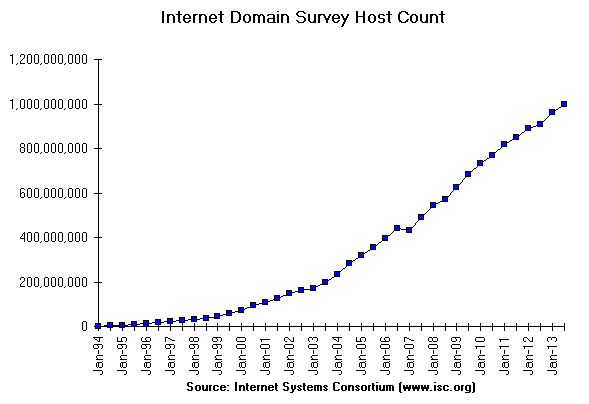
\includegraphics[scale=0.5]{./figures/hosts}
	\caption{L'évolution de nombre d'hôtes sur Interent de $1994$ à $2013$, cette figure  obtenues à partir de site: http://facesncups.com/inforev.html}
	\label{hosts}
\end{figure}
Par conséquent, si nous souhaitons modéliser ces réseaux, nous ne pouvons pas recourir à un modèle statique. Notre approche de modélisation doit plutôt reconnaître que les réseaux sont le produit d'un processus de croissance constant.
\begin{sloppypar}
\subsection{L'attachement préférentielle et le mécanisme "rich get richer"}
\end{sloppypar}
Le modèle des réseaux aléatoires suppose que nous choisissons au hasard les partenaires d'interaction d'un nœud. Pourtant, la plupart des réseaux réels les nouveaux nœuds préfèrent se lier aux nœuds les plus connectés, ce processus appelé attachement préférentiel. Par exemple, nous ne connaissons qu'une infime fraction du trillion ou plus de documents disponibles sur le WWW. Les nœuds que nous connaissons ne sont pas entièrement aléatoires: nous avons tous entendu parler de Google et de YouTube, mais nous rencontrons rarement les milliards de nœuds moins importants qui sont dans le Web. Comme nos connaissances sont biaisées vers les documents Web les plus populaires, nous sommes plus susceptibles de se lier à un nœud de haut niveau qu'à un nœud avec seulement quelques liens \cite{Barabasi2002}.\\
L'ancienneté, cependant, n'est pas suffisante pour expliquer la loi sans-échelle. Les Hubs nécessitent l'aide de la deuxième loi, l'attachement préférentiel. Parce que les nouveaux nœuds préfèrent se lier aux nœuds les plus connectés, les premiers nœuds avec plus de liens seront sélectionnés plus souvent et croîtront plus rapidement que les autres qui sont plus jeunes et moins connectés. Comme de plus en plus de nœuds arrivent et continuent de choisir les nœuds les plus connectés, les premiers nœuds vont inévitablement se détacher du paquet, acquérant un très grand nombre de liens. Ils vont se transformer en hubs. Ainsi, l'attachement préférentiel induit un phénomène "rich get richer" qui aide les nœuds les plus connectés à devenir plus connectés. Alors ce phénomène "rich get richer" mène naturellement aux lois sans-échelle observées dans les réseaux réels, nous allons confirmer cette idée dans la section suivante par notre propre travail et par une façons plus rigoureuse.
\begin{sloppypar}
\section{Attachement préférentiel sans l'effet "rich get richer"}
\end{sloppypar}
   %\subsection{Introduction}
   \subsection{Le modèle}
À l'instar du modèle BA original, notre réseau évolue selon deux mécanismes: la croissance et l'attachement préférentiel. Les nœuds entrant dans le réseau préfèrent s'attacher à des nœuds de faible degré, alors la probabilité $\Pi(k_i)$ que l'un des liens d'un nouveau nœud se connecte au nœud $i$ dépend de son degré $k_i$ tel que $\Pi(k_i)=C(1-\frac{k_i}{\sum_jk_j})$. où $C$ est la constante de normalisation.\\
En ce qui concerne les réseaux sociaux, si nous considérons le degré de nœuds comme décrivant la richesse des gens dans une société capitaliste, nous savons que nous vivons dans un monde où les riches s'enrichissent, mais quelle sorte de société nous aurons s' il n y a pas de faveur pour les gens riches, et il y a plutôt une subvention continue pour les pauvres ?
   
   Pour mettre en œuvre notre idée, nous commençons par $m_0$ nœuds, chacun avec $m$ liens. À chaque pas de temps, nous ajoutons un nouveau nœud avec $m$ arêtes qui lient le nouveau nœud à $m$ différents nœuds déjà présents dans le réseau. La probabilité que le nouveau nœud soit connecté à un noeud $i$ de degré $k_i$ est $\Pi(k_i)=C(1-\frac{k_i}{\sum_jk_j})$. La constante de normalisation $C$ est déduite de la condition $\sum_{i=1}^{t}\Pi(k_i)=1$, qui donne $C=\frac{1}{t+m_0-1}$. $t$ est l'instant auquel le dernier nœud a été créé et représente également le nombre de nœuds ajoutés au réseau.
   
   \subsection{Distribution des degrés en utilisant l'équation maîtresse}
   Notons $N(k,t)$ le nombre de nœuds de degré $k$ à l'instant $t$. La distribution des degrés à un instant donné $t$ sera écrite $P(k,t)=\frac{N(k,t)}{N(t)}$. Puisque à chaque pas de temps nous ajoutons un nouveau nœud au réseau, nous avons $N=t$. C'est, à tout moment, le nombre total de nœuds est égal au nombre de pas de temps.\\
   Nous écrivons l'attachement préférentiel dans notre modèle comme
   \begin{equation}
   \Pi(k)=C\big(1-\frac{k}{\sum_jk_j}\big)=C\big(1-\frac{k}{2mt+mm_0}\big)
   \end{equation}
   le terme $2m$ capture le fait que chaque lien contribue au degré de deux nœuds, et $mm_0$ capture le fait qu'à l'instant initial nous commençons par $m_0$ nœuds, chacun avec $m$ liens. Notre objectif est de calculer les changements dans le nombre de nœuds de degré $k$ après l'ajout d'un nouveau nœud au réseau. Pour cela, nous respectons les deux événements qui modifient $P(k,t)$ suite à l'arrivée d'un nouveau nœud:
   \begin{itemize}
   	\item Un nouveau nœud peut être lié à un nœud de degré $k$, le transformant en un nœud de degré $(k+1)$, ce qui diminue $P(k,t)$.
   	\item Un nouveau nœud peut être lié à un nœud de degré $(k-1)$, le transformant en un nœud de degré $k$, augmentant ainsi $P(k,t)$.
   \end{itemize}
  Alors pour ce modèle, l'équation maîtresse peut être écrite comme suit:
   \begin{equation}
   \begin{aligned}
  (t+1)P(k,t+1)= &tP(k,t)+m\Pi(k-1,t)tP(k-1,t)\\
   & -m\Pi(k,t)tP(k,t)+\delta_{k,m},
  \end{aligned}
 \end{equation}
  où $\delta$ est le symbole Kronecker.\\
  L'équation stationnaire correspondante prend la forme suivante:
  
  \begin{equation}
  \begin{aligned}
  (t+1)P(k)= &tP(k)+m\big(1-\dfrac{k-1}{2mt+mm_0}\big)\dfrac{tP(k-1)}{t-1}\\
  &-m\big(1-\dfrac{k}{2mt+mm_0}\big)\dfrac{tP(k)}{t-1} +\delta_{k,m},
  \end{aligned}
  \end{equation}
pour des temps très grand on peut écrire que $t+1=t$ et $t-1=t$, d'où
 \begin{equation}
 P(k)\big(1+m\big(1-\dfrac{k}{2mt+mm_0}\big)\big)=m\big(1-\dfrac{k-1}{2mt+mm_0}\big)P(k-1) +\delta_{k,m},
 \end{equation}
 après quelque lignes on obtient facilement que:
\begin{align}
P(k)&= 
\begin{cases}
\dfrac{2mt - (k-1)}{2t + 2mt - k}P(k-1), \quad \textrm{for }  k>m,\\
\\
\dfrac{2t}{2t + 2mt - m}, \quad\textrm{for }  k=m.
\end{cases}
\end{align}
La relation de récurrence ci-dessus donne la solution suivante:
\begin{align}
P(k)&= 
\begin{cases}
\dfrac{2t}{2t + 2mt - m}\prod^k_{j=m+1}\left( \dfrac{2mt -j + 1}{2t + 2mt - j}\right), \quad \textrm{for }  k>m,\\
\\
\dfrac{2t}{2t + 2mt - m}, \quad\textrm{for }  k=m.
\end{cases}
\label{eq4-2}
\end{align}
Bien que cette équation ne soit pas fermée, l'estimation numérique de $ P (k) $ est simple comme le montre Fig.~\ref{fig1-2}. \\
Nous simulons également le réseau avec des tailles allant jusqu'à $n=2\times10^6$, le nombre initial des nœuds est $m_0=3$ et $m=2$. 
Les résultats de la simulation confirment fortement les résultats analytiques (voir Fig.~\ref{fig1-2}). 

\begin{figure}[h]
	\centering
	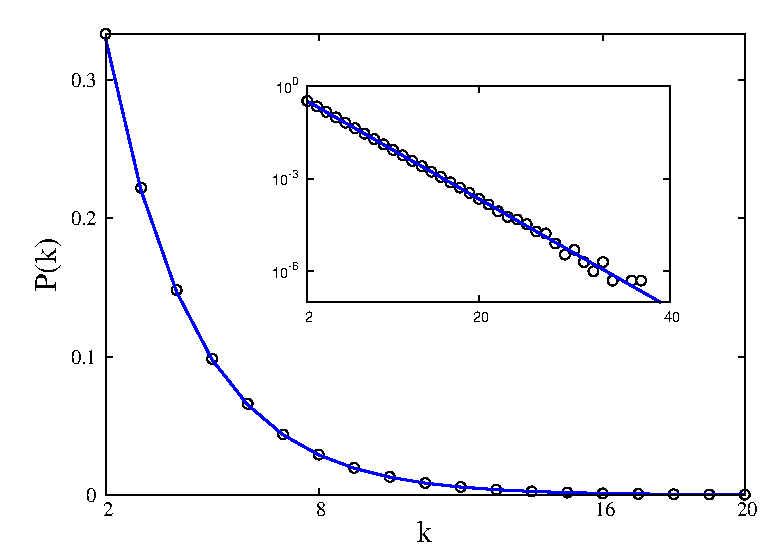
\includegraphics{./figures/fig1}
	\caption{les résultats de la simulation (cercles)  pour $n=2.10^6$, $m=2$, $m_0=3$, et la solution numérique (	ligne continue) pour Eq.~\eqref{eq4-2}. Dans l'encart, nous tracerons les mêmes données dans l'échelle log-linéaire.}
	\label{fig1-2}
 \end{figure} 
Nous avons observé dans les simulations que $k$ reste inférieur à $40$ pour $t=2.10^6$, nous prenons alors $t\gg j $ dans Eq.~\eqref{eq4-2} et nous obtenons
\begin{align}
P(k)&\approx 
\begin{cases}
\dfrac{1}{1+m}\Big(\dfrac{m}{1+m}\Big)^{k-m-1}, \quad \textrm{for }  k>m,\\
\\
\dfrac{1}{1+m}, \quad\textrm{for }  k=m.
\end{cases}
\label{eq5-2}
\end{align}
Après la normalisation, nous obtenons la distribution des degrés exponentielle $P(k)=Ae^{-A(k-m)}$, avec $A=\log(\dfrac{m+1}{m})$.
L'encart de la figure Fig.~\ref{fig1-2} montre la forme exponentielle de $ P(k)$ et l'excellent accord entre les simulations et les résultats théoriques.
Ceci confirme clairement que l'attachement préférentiel seul n'est pas suffisant pour produire des réseaux sans-échelle.

\subsection{Comparaison au niveau microscopique avec le modèle de BA}
 Nous recherchons les différences entre réseaux hétérogènes et homogènes en comparant notre modèle au modèle BA. La distribution des degrés ne suffit pas à elle seule à caractériser les réseaux. Le calcul d'autres quantités microscopiques peut aider à mieux comprendre leur évolution et leur formation. Il s'avère que le réseau sans-échelle a des nœuds avec un degré important (hubs), tandis que le réseau aléatoire n'a pas de structure apparente. L'évaluation du degré moyen instantané du nœud cible $\kms$ et de ses fluctuations peut fournir des informations quantitatives sur les nœuds du réseau. En fait, $\kms$ est en quelque sorte lié au degré moyen instantané des hubs, car lors du choix aléatoire des nœuds, les hubs ont plus de chance d'être sélectionnés. \\  
 Dans un premier temps, nous analysons $\kms$ et $\kmss$ dans le réseau BA
 \begin{eqnarray}
 \kms=\sum_{t_i=1}^t\Pi(k_i)k_i(t)+m_0\Pi(k_0)k_0(t),
 \label{eq6-2}
 \end{eqnarray}
 où  $\Pi(k_i)=\frac{k_i(t)}{2mt+mm_0}$, $t_i$ est l'instant auquel le nœud $ i $ a été créé et $ k_0 (t) $ est le degré des nœuds initiaux à l'instant $t$.\\
 $k_i (t)$ est facilement calculé à partir de l'équation d'évolution du degré de champ moyen:
 $\dfrac{\partial k_i(t)}{\partial t}=~ m\Pi(k_i)$, qui donne $k_i(t)=m\Big(\frac{2t+m_0}{2t_i+m_0}\Big)^{\frac{1}{2}}$.\\
 En insérant la dernière expression dans l'Eq.~\eqref{eq6-2}, on obtient
 \begin{eqnarray}
 \kms&=&m\Big(\sum_{t_i=1}^{t}\dfrac{1}{2t_i+m_0}+1\Big) \\
 &=&m \Big(\ln (2t+m_0)+\gamma-a+\frac{1}{2(2t+m_0)}+O(\frac{1}{t^2})\Big),
 \label{eq7-2}
 \end{eqnarray}
 où $\gamma$ est la constante d'Euler, et $a=\frac{1}{2}+\frac{1}{3}+\ldots+\frac{1}{1+m_0}$.\\
 Un bon accord est obtenu comme le montre la figure Fig.~\ref{fig2a-2} entre Eq.~\eqref{eq7-2} et les résultats de la simulation même pour les premiers instants de l'évolution. $\kms$ croît indéfiniment avec le temps et diverge pour un réseau infini (oo $t\to\infty$) du fait que, dans les réseaux hétérogènes, les hubs sont plus susceptibles d'être sélectionnés et liés aux nouveaux nœuds. \\
 De l'autre côté, le degré moyen du réseau reste fini \cite{Barrat-a2008l,Cohen-Havlinl2010} puisque la majorité des nœuds ont un faible degré et le poids des hubs est faible.\\
 \begin{figure}[h]
 	\centering
  	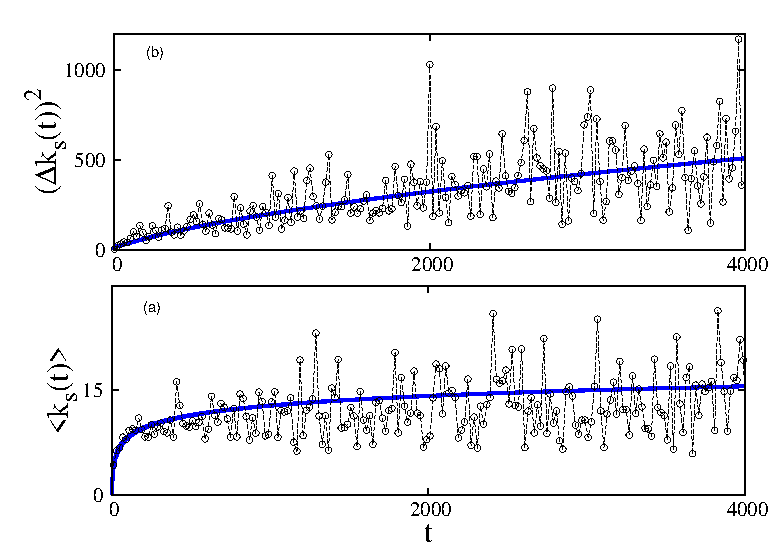
\includegraphics[scale=0.85]{./figures/nfig2}
 	\caption{(a) Évolution de $\kms$ dans le modèle BA, la ligne continue représente Eq.~\eqref{eq7-2}.
 	(b) Évolution des fluctuations de $\kms$, la ligne continue représente Eq.~\eqref{eq10-2}. Les cercles joints par des lignes pointillées dans les deux cas sont des données de simulation moyennées sur 20 réalisations pour $m =2$, $m_0=3$.}
 	\label{fig2a-2}
 \end{figure}
 
 Le deuxième moment $\kmss$ s'écrit
 \begin{align}
 \kmss&=\sum_{t_i=1}^t\Pi(k_i)k^2_i(t)+m_0\Pi(k_0)k_0^2(t)\label{eq8-2} \\
 &\approx m^2(2t+m_0)^{\frac{1}{2}} \Big(\sum_{t_i=1}^t \frac{1}{(2t_i+m_0)^{\frac{3}{2}}}+m_0^{-\frac{1}{2}}\Big).
 \end{align}
 Pour des grands temps, $\sum_{t_i=1}^t\Big(\frac{1}{t_i}\Big)^{\frac{3}{2}}=\zeta(\frac{3}{2}) \approx 2.612$, on obtient 
 \begin{eqnarray}
 \begin{split}
 \kmss&\approx m^2\sqrt{2t}(m_0^{-\frac{1}{2}}+2.612-b),
 \label{eq9-2}
 \end{split}
 \end{eqnarray}
où $b=1+\frac{1}{2^\frac{3}{2}}+\frac{1}{3^\frac{3}{2}}+\ldots+\frac{1}{(1+m_0)^\frac{3}{2}}$.\\
Fluctuations de $\kms$ sont donnés par
\begin{align}
(\Delta k_s(t))^2 \equiv \kmss-\kms^2\approx m^2 \Big[(m_0^{-\frac{1}{2}}+2.612-b)\sqrt{2t}-(\ln(2t))^2\Big],
\label{eq10-2}
\end{align}
qui deviennent arbitrairement large lorsque le temps augmente suffisamment. \\
Les données de simulation selon Eq.~\eqref{eq10-2} ( voir Fig.~\ref{fig2a-2}(b)) montrent la tendance croissante des fluctuations de $\kms$.
Cela peut s'expliquer par le fait que le degré maximum dans le réseau $k_{max}\sim \sqrt{t}$ \cite{Cohen-Havlinl2010} augmente plus vite que $\kms\sim \ln(t)$ (Eq.~\eqref{eq7-2}) et la différence entre les deux quantités devient plus grande avec le temps. \\
Nous passons maintenant à la même analyse dans notre modèle,  L'équation d'évolution du champ moyen pour $k_i(t)$ est donnée par
\begin{eqnarray}
\dfrac{\partial k_i(t)}{\partial t}=m\Big(1-\dfrac{k_i(t)}{2mt+mm_0}\Big)\dfrac{1}{t+m_0-1},
\end{eqnarray}
La solution a la forme
\begin{eqnarray}
k_i(t)=m \Big(\frac{t+m_0-1}{2t+m_0}\Big)^{\frac{1}{m_0-2}}\Bigg[\Big(\frac{t_i+m_0-1}{2t_i+m_0}\Big)^{-\frac{1}{m_0-2}}-A(t_i)
+A(t)\Bigg],
\label{kit}
\end{eqnarray}
où $A(t)=\displaystyle \int_1^{t}\dfrac{\Big(\frac{t'+m_0-1}{2t'+m_0}\Big)^{-\frac{1}{m_0-2}}}{t'+m_0-1}dt'$.\\
On sait que la valeur moyenne du nœud sélectionné $\kms$ est sous la forme 
\begin{eqnarray}
\kms=\sum_{t_i=1}^t\Pi(k_i)k_i(t)+m_0\Pi(k_0)k_0(t),
\label{kms-2}
\end{eqnarray}
 en remplaçant Eq.~\eqref{kit} dans cette dernière équation on obtient immédiatement pour tout temps $ t $ l'expression de $\kms$, L'équation résultante est résolue numériquement comme le montre Fig.~\ref{fig2b-2}. \\
Pour les temps très grands et en prenant $t \gg m_0$, nous trouvons 
$A(t)\approx 2^{\frac{1}{m_0-2}} \ln(t)$, $k_i(t)\approx m\Big(1+\ln \dfrac{t}{t_i}\Big)$, d'où
\begin{align}
\label{kom}
\kms&\approx\dfrac{m}{t}\Big(\sum_{t_i=1}^{t} \ln(t)-\ln(t_i)+1\Big)\\
&\approx\dfrac{m}{t}\Big(t \Big(\ln(t)+1\Big)-\Big(\sum_{t_i=1}^{t} \ln(t_i)\Big)\Big) \nonumber \\
&\approx\dfrac{m}{t}\Big(t\ \Big(\ln(t)+1\Big)-\ln(t_i!)\Big) \nonumber \\
&\approx2m. \nonumber
\end{align}

Le second moment est obtenu en substituant les expressions correspondantes de $\Pi(k_i)$ et $k_i(t)$ dans Eq.~\eqref {eq8-2}, nous obtenons pour les temps très grands
 \begin{eqnarray}
\begin{split}
\kmss\approx \frac{m^2}{t}\Big(\sum_{t_i=1}^t (\ln(\frac{t}{t_i})+1)^2\Big).
\label{k2om}
\end{split}
\end{eqnarray}
Faire les approximations  $\sum_{t_i=1}^t \ln(t_i)\approx t\ln(t)-t$, et
$\sum_{t_i=1}^t \ln(t_i)^2\approx t\ln(t)^2-2t\ln(t)+2t-2$, on obtient $\kmss\approx 5m^2.$ Fluctuations sont 
\begin{eqnarray}
 (\Delta k_s(t))^2 \equiv {\kmss-\kms^2}\approx m^2.
\end{eqnarray}
 Ce résultat, additionné avec $\kms\approx 2m $, montrent que presque tous les nœuds ont le même degré que celui illustré sur Fig.~\ref{fig2b-2}. L'homogénéité du réseau peut s'expliquer par le fait que l'attachement préférentiel utilisé ici ne permet pas la formation des hubs, puisqu'il ne permet pas aux riches de s'enrichir, ni d'enrichir les pauvres. 
\begin{figure}[h]
	\centering
	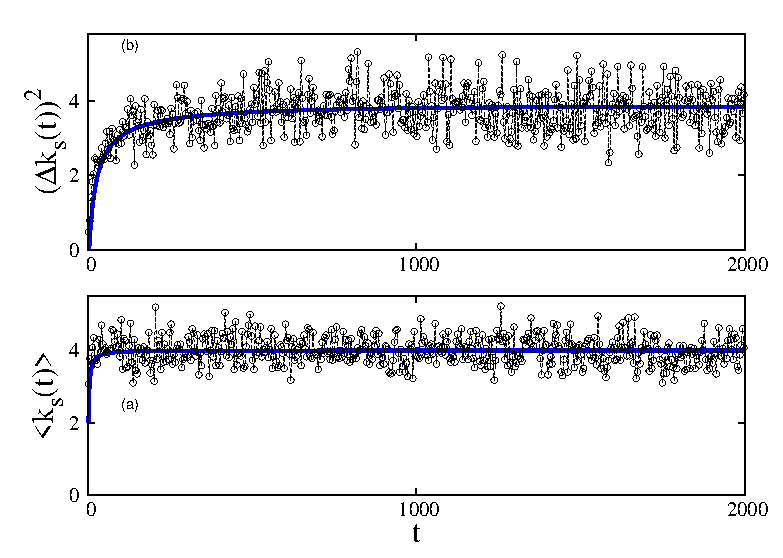
\includegraphics[scale=1]{./figures/nfig3}
	\caption{(a) Évolution de $\kms$ dans notre modèle, la ligne continue représente Eq.~\eqref{kms-2}.
	(b) Évolution des fluctuations de $\kms$, la ligne continue représente la solution numérique de Eq.~\eqref{kms-2} et Eq.~\eqref{k2om}. Les cercles joints par des lignes pointillées dans les deux cas sont des données de simulation moyennées sur $20$ réalisations pour $m=2$, $m_0=3$.}
	\label{fig2b-2}
\end{figure}
 \vspace{4cm}
\section{conclusion}

Dans ce chapitre, nous avons commencé par donner quelques idées sur les processus dynamiques, l'attachement préférentiel et le mécanisme "rich get richer" dans les réseaux réels , puis nous avons introduit un simple modèle de réseau complexe avec un critère d'attachement préférentiel et sans effet "rich get richer". Le réseau obtenu est homogène, ce qui démontre le rôle crucial du "rich get richer" dans la topologie du réseau, en outre nous avons conclu que le fait de donner un traitement préférentiel aux nœuds les moins connectés équivaut à utiliser une probabilité d'attachement aléatoire. \\
Le Calcul du degré moyen instantané d'un nœud sélectionné et ses fluctuations fournissent plus d'informations que le degré moyen habituel du réseau, en particulier nous avons montré comment le degré moyen des hubs et ses fluctuations divergent avec le temps dans le modèle BA, et restent finis dans notre modèle.
%En termes de répartition de la richesse sociale, le principe de Pareto \cite{Pareto1897} ne s'applique pas et nous avons plutôt une distribution exponentielle du revenu.